\documentclass[a4paper,11pt]{article}
\renewcommand{\baselinestretch}{1.5}
\usepackage{graphicx}
\graphicspath{{.}{../results_plots/}}
\usepackage{siunitx}
\usepackage{amstext, amsmath, amssymb,color}
\usepackage[colorlinks=true,linkcolor=blue]{hyperref}
\usepackage{subcaption}
\usepackage[a4paper, left=2.5cm, right=2.5cm, top=1.8cm, bottom=1.8cm, includehead, includefoot, head=30pt]{geometry}
\newtheorem{thm}{Theorem}
\usepackage{pdflscape}

%\renewenvironment{proof}{{\bfseries Proof }} {\qed}

\title{Bias reduction in tail estimation and modelling a full data set}
\author{ J. Beirlant $^{a,b}$\footnote{Corresponding author: Jan Beirlant, KU Leuven, Dept of Mathematics, Celestijnenlaan 200B, 3001 Heverlee, Belgium; Email: jan.beirlant@kuleuven.be }, G. Maribe $^{b}$,  Ph. Naveau$^{c}$, A. Verster$^{b}$  \\
{\fontsize{8pt}{11pt} \selectfont $^a$ Dept. of Mathematics, LStat and LRisk, KU Leuven}
\\
{\fontsize{8pt}{11pt} \selectfont $^b$ Dept. of Mathematical Statistics and Actuarial Science, Free State University }
\\
{\fontsize{8pt}{11pt} \selectfont $^c$ Laboratoire des Sciences du Climat et de l'Environnement, CNRS, Universit\'e Paris-Saclay}
%    General info
%\subjclass[2000]{Primary 62G32; secondary 60G70, 62P05, 62P12,
%92F05}
%\date{24/08/2009}
}
\begin{document}

 
\maketitle
\begin{abstract}
{\noindent In recent years several attempts have been made to model both the modal and tail part of the data. 
Frigessi et al. (2002) proposed dynamic mixtures of two components with a weight function $\pi=\pi (x)$ smoothly connecting the bulk and the tail of the distribution. 
Recently,  Naveau et al. (2016) propose a nice review on this topic, and, continuing on the work by Papastathopoulos and Tawn (2013), propose a statistical model which is in compliance with extreme value theory and allows for a smooth transition  between the modal and tail part.
Incorporating second order rates of convergence for distributions of peaks over thresholds, Beirlant et al. (2002, 2009) constructed  models that can be viewed as special cases from both approaches discussed above. When fitting such second order models it turns out that the bias of the resulting extreme value estimators is significantly reduced compared to the fit with one Pareto component. Recently, Beirlant et al. (2017) showed that using penalized likelihood methods on the weight parameter one can obtain good bias and mean squared error properties for tail estimators. In this paper we encompass the above approaches providing models that can be used to model full data sets, that comply with extreme value theory, and that provide appropriate tail fits with special attention for tail estimation with reduced bias and mean squared error under the classical max-domain of attraction conditions.
 }
\end{abstract}

\noindent {\bf Keywords:} Generalized Pareto distribution; Tail estimation; Mixture models; Shrinkage estimators.

%\noindent {\bf AMS 2000 subject classifications.} 62G32, %62H12, 62G20.



%%\begin{document}

\section{Introduction} 
\label{Sec1}              % --- this section label

In recent literature, several attempts have been made to combine tail modelling using extreme value methodology with models that are able to capture the characteristics of the bulk of the data. Extreme value (EV) methodology starts from the assumption that the distribution function $F$ underlying the data $X_1, X_2,\ldots,X_n$ belongs to the domain of attraction of a generalized extreme value distribution, i.e.  there exists sequences $(b_n)_n$ and $(a_n>0)_n$ such that as $n \to \infty$
\begin{equation}
{\max (X_1, X_2,\ldots,X_n)-b_n \over a_n} \to _d Y_{\xi},
\label{maxd}
\end{equation}
where $\mathbb{P} (Y_\xi >y) = \exp (-(1+\xi y)^{-1/\xi})$, for some $\xi \in \mathbb{R}$. The parameter $\xi$ is termed the extreme value index (EVI). It is well-known that \eqref{maxd} is equivalent to the existence of a positive function $t \mapsto \sigma_t$, such that 
\begin{equation}
\mathbb{P}\left({X-t \over \sigma_t} >u| X>t \right)
= {1-F(t+u\sigma_t) \over 1-F(t)} \to_{t \to x_+}
\bar{H}^{GP}_{\xi}(u)= (1+\xi u)^{-1/\xi},  
\label{POT}
\end{equation}
where $x_+$ denotes the endpoint of the distribution of $X$. The conditional distribution of $X-t$ given $X>t$ is called the peaks over threshold (POT) distribution, while $\bar{H}_{\xi}$ is the survival function of the generalized Pareto distribution (GPD).\\
In case $\xi >0$, the limit in \eqref{maxd} holds if and only if $F$ is of Pareto-type, i.e.
\begin{equation}
1-F(x) = x^{-1/\xi}\ell (x),
\label{Patype}
\end{equation} 
for some slowly varying function $\ell$, i.e. satisfying $\frac{\ell(ut)}{\ell (t)} \to 1 $ as $t \to \infty$, for every $u>1$. Pareto-type distributions satisfy a simpler POT limit result: as $t \to \infty$
\begin{equation}
\mathbb{P} \left( {X \over t} >u | X>t \right) \to \bar{H}^P_{\xi}(u) := u^{-1/\xi}, u>1. 
\label{POTPa}
\end{equation}

Estimation of $\xi$, and tail probabilities or tail quantiles, is then based on fitting a GPD to the observed excesses $X-t$ given $X>t$, respectively a simple Pareto distribution with survival function $u^{-1/\xi}$ to $X/t$ given $X>t$ in case $\xi >0$.
The main difficulty in such an EV application is the choice of the threshold $t$. Most often, the threshold $t$ is chosen as one of the top data points $X_{n-k,n}$ for some $k \in \{1,2, \ldots,n \}$ where $X_{1,n} \leq X_{2,n} \leq \ldots X_{n,n}$ denotes the ordered sample. The limit result in \eqref{POT} and \eqref{POTPa} require $t$ to be chosen as large as possible (or, equivalently, $k$ as small as possible for the bias in the estimation of $\xi$ and other tail parameters to be limited. However, in order to limit the estimation variance, $t$ should be as small as possible, i.e. the number of data points $k$  used in the estimation should be as large as possible. Several adaptive procedures for choosing $t$ or $k$ have been proposed, but mainly in the Pareto-type case with $\xi >0$, see for instance Chapter 3 in Beirlant et al. (2004), or Matthys and Beirlant (2000). \\
In case of a real-valued EVI, the selection of an appropriate threshold is even more difficult and only a few methods are available. Dupuis (1999) suggested a robust model validation mechanism  to guide the threshold selection, assigning weights between 0 and 1 to each data point where a high weight means that the point should be retained since a GPD model is fitting it well. However, thresholding is required at the level of the weights and hence the method cannot be used in an unsupervised manner. 
\\

Another approach consists of proposing penultimate limit distributions in \eqref{POT} and \eqref{POTPa}. In case $\xi >0$, Beirlant et al. (2009) proposed the extended Pareto distribution (EPD) as an improved approximation of the distribution of $X/t$ given $X>t$ as $t \to \infty$ with survival function
\[
 \left\{u (1+ \kappa_t -\kappa_t u^{-\beta}) \right\}^{-1/\xi} 
,
\]
with $\beta >0$ and $\kappa_t$ satisfying $\delta_t \downarrow 0$ as $t \to \infty$, leading to the approximation
\begin{equation}
\bar{H}_{\xi}^{EP}(u) := u^{-1/\xi}\left( 1- \delta_t + \delta_t (u^{-1/\xi})^{\beta\xi}\right).
\label{EP}
\end{equation}

 This model is derived from the mathematical theory of second order slow variation, under which 
\begin{equation}
\frac{\ell(ut)}{\ell (t)} - 1 =\kappa_t 
\left( u^{-\beta}-1 \right),
\label{SO}
\end{equation}
where $\kappa_t=\kappa (t)= t^{-\beta}\tilde{\ell}(t)$, with $\tilde\ell$ slowly varying at infinity (see section 2.3 in de Haan and Ferreira, 2006). {\it Note  that such a mixture model  $H_{\xi}^{EP}$ will improve the approximation of  $\left( {X \over t} >u | X>t \right)$ for values of $t$ which are smaller than the appropriate $t$-values when estimating the POT with $H_{\xi}^{P}$. On the other hand one cannot expect this extended Pareto distribution to approximate POT distributions for the lowest thresholds $t$, and hence then it cannot provide an appropriate model for the full sample.} 
\\
In Beirlant et al. (2009), using an external estimator  of $\rho=-\beta\xi$, the parameters $(\xi, \delta)$ are estimated fitting the EPD by maximum likelihood on excesses over a random threshold $X_{n-k,n}$, $k=1,2,\ldots,n$. 
The result of this procedure are two-fold:
\begin{itemize}
\item First, as a function of $k$, the estimates $\hat{\xi}_k^{EP}$ of $\xi$ are much more stable compared to the original ML estimator proposed by Hill (1975)
$$
H_{k,n} = {1 \over k} \sum_{j=1}^k \log {X_{n-j+1,n}\over X_{n-k,n}}
$$
 which is obtained by fitting the Pareto distribution to the excesses 
 $\{ {X_{n-j+1,n}\over X_{n-k,n}}, j=1,\ldots,k\}$ following \eqref{POTPa}. Indeed, the bias in the simple POT model \eqref{POTPa} is estimated and it is shown that, under the assumption that the EP model for the excesses $X/t$ is correct and that $\beta$ is estimated consistently,  the asymptotic bias of  $\hat{\xi}_k^{EP}$ is 0 as long as  $k (k/n)^{2\beta\xi} \to \lambda >0$ as $k,n \to \infty$, while the asymptotic bias of $H_{k,n}$ is only 0 when $k (k/n)^{2\beta\xi} \to 0$.
 \item On the other hand,  the asymptotic variance of $\hat{\xi}_k^{EP}$ equals $((1-\rho)/\rho)^2 {\xi^2 \over k}$, where ${\xi^2 \over k}$ is the asymptotic variance of $H_{k,n}$. 
\end{itemize}
Bias reduction techniques in the Pareto-type case $\xi >0$ have also been proposed, among others in Feuerverger and Hall (1999), Gomes et al. (2000), Beirlant et al. (1999, 2002) and Gomes and Martins (2002). In Caeiro and Gomes (2011) methods are proposed to limit the variance of bias-reduced estimators to the level of the variance of the Hill estimator $H_{k,n}$. The price to pay is then to assume a third-order slow variation model specifying \eqref{SO} even further. These methods focus on the distribution of the $\log$-spacings of high order statistics.  Other ad hoc construction methods for asymptotically unbiased estimators of $\xi >0$ were introduced in Peng (1998) and Drees (1996).
\\

In order to keep the variance under control for small values of $k$, Beirlant et al. (2017) proposed to use a shrinkage estimator for $\delta$, putting a penalty on $\delta$ forcing the estimator of this parameter to tend to 0 for large values of $t$. When using the mathematical fact that  $\delta_t \to 0$ as $t \to \infty$ in the statistical estimation procedure, Beirlant et al. (2017) constructed  a dynamically weighted mixture model in the spirit of Frigessi et al. (2003): the weights $\delta_t$  vary in such a way that for large values of $t$, the simple Pareto component $u^{-1/\xi}$ is predominant and hence these weights take over the role of threshold selection. A similar mixture of two Pareto components was proposed in Peng and Qi (2004). 
Such dynamic mixture  model also allows to enhance {\it the fit of the full data set} (next to the part of the data above the threshold $t$), which is also important in many applications.
\\

In the general case $\xi \in \mathbb{R}$, considering all max-domains of attraction, the literature on bias reduction and/or full model construction is much more limited. Frigessi et al. (2002) proposed the mixture model with density
\[
f(x) = \frac{p(x;\theta_1)h_{\xi}({x \over \sigma}) + (1-p(x;\theta_1))f(x;\theta_2)}{Z(\theta_1, \theta_2,\xi, \sigma)},
\]
where $h_{\xi}(y) =(1+\xi y)^{-1-1/\xi }$ denotes the GPD density, 
and with $p(x;\theta_1)$ a mixing function taking values in $[0,1]$ increasing in $x$, and $Z$ denoting the normalizing constant. More specifically, these authors selected $p(x;\theta_1) = {1 \over 2} + {1 \over \pi}\mbox{arctan}\left( {x -\mu \over \tau} \right)$ ($\theta_1= (\mu,\tau)$) and the Weibull distribution for $f(x; \theta_2)$. \\
Recently, Naveau et al. (2016), generalizing Papastathopoulos and Tawn (2013),  proposed to use full models for rainfall intensity data that are able to capture low, moderate and heavy rainfall intensities without a threshold selection procedure. These authors propose to model all data jointly using transformation models with survival function 
\begin{equation}
F(x) =  G_0 (H_{\xi} \left({x \over \sigma})\right),
\label{naveau}
\end{equation}
with $G_0$ a distribution function on $[0,1]$, satisfying constraints to preserve the classical tail GPD fit and a power behaviour for small rainfall intensities:
\begin{itemize}
\item $\lim_{v \downarrow 0} \frac{1-G_0(1-v)}{v}=a$, for some $a>0$,
\item $\lim_{v \downarrow 0} \frac{G_0(v w(v))}{G_0(v)}=b$, for some $b>0$ where $v \mapsto w(v)$ is a positive function satsfying $w(v) = 1+ o(v)$ as $v \to 0$,
\item  $\lim_{v \downarrow 0} \frac{G_0(v)}{v^\kappa}=c$, for some  $c>0$ and $\kappa >0$.
\end{itemize}
Examples of $G$ functions  are $G(v)= v^\kappa$ or 
$G(v) = 1-{1+D \over D} (1-v) (1-\frac{(1-v)^D}{1+D})$, $v \in (0,1)$. 
In Naveau et al. (2017) this model is further elaborated approximating $G_0$ using Bernstein polynomials of degree $m$, i.e. using $G_{0}^{(m)} (u) = \sum_{j=0}^m G({j \over m})b_{j,m}(u)$ with $b_{j,m}(u)$ the binomial ($m,u$) mass density at $j$.  
\\
In Naveau et al. (2016, 2017) the primary goal is the search for a model fitting the whole outcome set, 
while the fit of the proposed model to POT values $X-t |X>t$ for extrapolation purposes in order to estimate extreme quantiles and tail probabilities is imposed using the condition $\lim_{v \downarrow 0} \frac{1-G_0(1-v)}{v}=a$. However the bias and MSE properties of the estimators of $\xi$ and $\sigma$ still have to be analyzed.\\

In this paper we propose a compromise between the Frigessi et al. (2002) and Naveau et al. (2016,2017)  approach, fitting models with survival functions of the type
\begin{equation}
G_t \left(\bar{H}^{GP}_{\xi}({x \over \sigma})\right)
=
\bar{H}^{GP}_\xi ({x \over \sigma})\left\{1-\delta_t +\delta_t \phi_{\theta}\left( \bar{H}_\xi ( {x \over \sigma}) \right) \right\},
\label{FM}
\end{equation} 
to the POTs $X-t|X>t$, with 
\begin{itemize}
\item $\delta_t =\delta (t) \to 0$ as $t \to x_+$,
\item $\delta_t =\delta (t) \uparrow 1$ as $t  \to 0$,
\item $u \mapsto u\phi_\theta (u)$ a distribution function concentrated on $(0,1)$.
\end{itemize}
For negative $\delta$-values one needs $\delta_t > \{\min_u (1-{d \over du}\, (u\phi_\theta (u))\}^{-1}$ to obtain a valid distribution.  
  At $t=0$ the function $u\phi_{\theta}(u)$ then corresponds to $u \mapsto 1-G(1-u)$ in \eqref{naveau}, while as $t \to \infty$ this is the case for the GPD survival function $\bar{H}_\xi (x/\sigma)$.
  \\\\  
 This proposal can be viewed as an extension of  the second-order regular variation condition in terms of distribution functions, i.e. 
 \begin{equation}
 \lim_{t \to x_+}{ {1-F(t+u\sigma_t) \over 1-F (t)}- (1+\xi u)^{-1/\xi} \over \alpha (t)} = (1+\xi u)^{-1-1/\xi}B_{\xi,\tilde{\rho}}((1+\xi u)^{1/\xi}),
 \label{secondorder}
 \end{equation}
 with $\alpha(t) \to 0$ as $t \to x_+$, $B_{\xi,\tilde{\rho}}(x)= {1 \over \tilde\rho}\left({x^{\xi +\tilde{\rho}}-1 \over \xi +\tilde\rho}- {x^{\xi}-1 \over \xi}\right)$ for some $\tilde\rho \leq 0$ (see for instance Theorem 2.3.8 in de Haan and Ferreira, 2006. For the cases $\xi+\tilde\rho=0$ and $\xi=0$ this is understood to be equal to the limit of $B$ as these parameters tend to 0. When $\xi+\tilde\rho \neq 0$ and $\tilde\rho<0$, this second-order condition leads to  a special case of \eqref{FM} with $\delta_t = \alpha_t/(\xi\tilde{\rho})$,  $\phi_\theta (u) = u^{-\xi} {\tilde{\rho} \over \xi +\tilde{\rho}}+  u^{-\tilde{\rho}} {\xi \over \xi +\tilde{\rho}}$ and $\theta= (\xi,\tilde\rho)$. This particular example then allows for bias reduced estimation of $(\xi,\sigma)$ under the assumption that the second order model \eqref{secondorder} is a correct model for the POTs $X-t|X>t$. In this sense, model \eqref{FM} when used as a model for POTs $X-t|X>t$, generalizes the approach taken in Beirlant et al. (2009) and Beirlant et al. (2017) to all domains of attraction. When \eqref{FM} is used as a model for all observations, taking $t=0$, this model directly encompasses the models from Frigessi et al. (2002) 	and Naveau et al. (2016).\\
 
 Of course this approach can also be applied to the specific case of Pareto-type distributions ($\xi >0$) approximating the distribution of POT values $X/t|X>t$ using models of the type
 \begin{equation}
G_t \left(\bar{H}^P_{\xi}(x)\right)
=
\bar{H}^P_\xi (x)\left\{1-\delta_t +\delta_t \phi_{\theta}\left( \bar{H}^P_\xi ( x) \right) \right\},
\label{FM+}
\end{equation} 
with the EPD model \eqref{EP}  as a special case with $\phi_{\theta}(u)=u^{\beta\xi}$.\\
 
 In this paper, using the Bernstein polynomial approach from Naveau et al. (2017), we will study
 \begin{itemize}
 \item the estimation procedure fitting \eqref{FM}, or \eqref{FM+} in case $\xi >0$, to high thresholds $t$ deriving the asymptotic distribution of the corresponding ML estimators when $k,n \to \infty$ and $k/n \to 0$, given an appropriate choice of $ \phi_\theta$;
  \item the finite sample goodness-of-fit behaviour of the full model obtained from fitting model \eqref{FM} to all data;
  \item the effect of penalized estimation of $\delta_t$ forcing $\delta_t \to 0$ as $t \to \infty$. 
 \end{itemize}
 
 \section{The estimation procedure}
 
 Here we propose to build the estimation procedure on the Bernstein polynomial approximation procedure from Naveau et al. (2017) constructing $G_{0,m}$ from which $\phi_{\theta}$ can be constructed. The survival function $1-F_t$ of the POTs at threshold $t$ is then approximated through
 \begin{eqnarray*}
 1-\hat{F}_t(x) &=& 1- G_{0,t}^{(m)}\left(1-\bar{H}^{\bullet}_{\xi}(x)\right) \\
 &=& G_{t}^{(m)}\left( H^{\bullet}_{\xi}(x) \right). 
  \end{eqnarray*} 
 where $\bar{H}^{\bullet}$ refers to the generalized Pareto (GP) or the Pareto (P) distribution as appropriate, and $G_{t}^{(m)}(u)=1-G_{0,t}^{(m)}(1-u)$. 
 One can then obtain a Bernstein approximation $\hat{G}_{0,t}^{(m)}$ of degree $m$ obtaining the corresponding density 
 $\hat{g}_{0,t}^{(m)}(v) = \sum_{j=1}^m  \hat{\omega}_{j,m,t}\beta_{j,m-j+1}(v)$ where $\beta_{j,m-j+1}(v)= (B(j,m-j+1))^{-1}v^{j-1}(1-v)^{m-j} $ are Beta densities and where
 $\hat{\omega}_{j,m,t}= \hat{G}({j \over m})-\hat{G}({j-1 \over m})$. The linear coefficient in $\hat{G}_t^{(m)}$ is then given by $m\hat{\omega}_{m,m,t}$ so that we can write
 \begin{eqnarray}
 1-\hat{F}^{\bullet}_t(x) &=& 
\bar{H}_{\xi}^{\bullet}(x)\, m\hat{\omega}_{m,m,t} + (1-m\hat{\omega}_{m,m,t}){ \hat{G}^{(m)}_t(\bar{H}^{\bullet}_{\xi}(x))-\bar{H}^{\bullet}_{\xi}(x)m\hat{\omega}_{m,m,t} \over 1-m\hat{\omega}_{m,m,t}}\\
&=& \bar{H}^{\bullet}_{\xi}(x) \left\{
m\hat{\omega}_{m,m,t} + (1-m\hat{\omega}_{m,m,t}){ \hat{G}^{(m)}_t(\bar{H}^{\bullet}_{\xi}(x))-\bar{H}^{\bullet}_{\xi}(x)m\hat{\omega}_{m,m,t} \over \bar{H}^{\bullet}_{\xi}(x) (1-m\hat{\omega}_{m,m,t})}
\right\} \\
&=& \bar{H}^{\bullet}_{\xi}(x) \left\{ (1-\hat{\delta}_t) 
+ \hat{\delta}_t \, \hat{\phi}_{\theta} \left( \bar{H}^{\bullet}_{\xi}(x)\right)\right\} 
 \end{eqnarray}
 with $\hat{\delta}_t = 1-m\hat{\omega}_{m,m,t}$ and $(1-m\hat{\omega}_{m,m,t}) \, u \hat{\phi}_{\theta}(u) =  \hat{G}^{(m)}_t(u)-u \, m\hat{\omega}_{m,m,t} $ referring to the Bernstein approximation of $G_t^{(m)}$ without the first degree term. \\
 
 Given a value of $m$ and at every $t$, penalized maximum likelihood estimation of $(\xi,\sigma)$ in case $\xi \in \mathbb{R}$ (or $\xi$ in case one restricts to $\xi >0$) is then combined with the estimation of the coefficients $\hat{\omega}_{j,m,t}$ ($j=1,\ldots,m$) in the following way ....
 \newpage
We apply the algorithm of Naveau et al. (2017) with a slight modification to the log-likelihood. In estimating $\theta = (\sigma, \xi)$ we add a quadratic penalty to the log-likelihood and solve;
\begin{eqnarray}
\boldsymbol{\hat{\theta}}^{MLE} = \text{argmin}\left\{\sum_{i=1}^{n}\log (\hat{g}_{m,n}\{H_{\xi}(x_i)\})+\sum_{i=1}^{n}\log \{h_{\xi}(x_i)\} + \lambda \frac{(1-m\omega_{m,m})^2}{2k\sigma_{k,n}^2}\right\}
\end{eqnarray}where $\lambda$ is a tunning parameter regulating the amount of penalty enforced on $1-m\omega_{m,m}$. For now, we use the rate $\sigma_{k,n}^2=(k/n)^{-2\rho}$.

$m$ is chosen at $n-1$ and fixed for all $k$, for every $k$ however new estimates of $\boldsymbol{\theta}$ are computed and iteratively used to compute new weights with a penalty enforced on the last omega.
The choice of $m$ can in the case of simulations be chosen through the Mean integrated square error, mean integrated absolute error or method of least square cross validation. As noted by Naveau et al. (2017), the latter method is advantageous since in practice, since we do not know the true distribution of the data.
 
 \section{Simulations and case study}
 
 \begin{figure}[!ht]
  \centering
 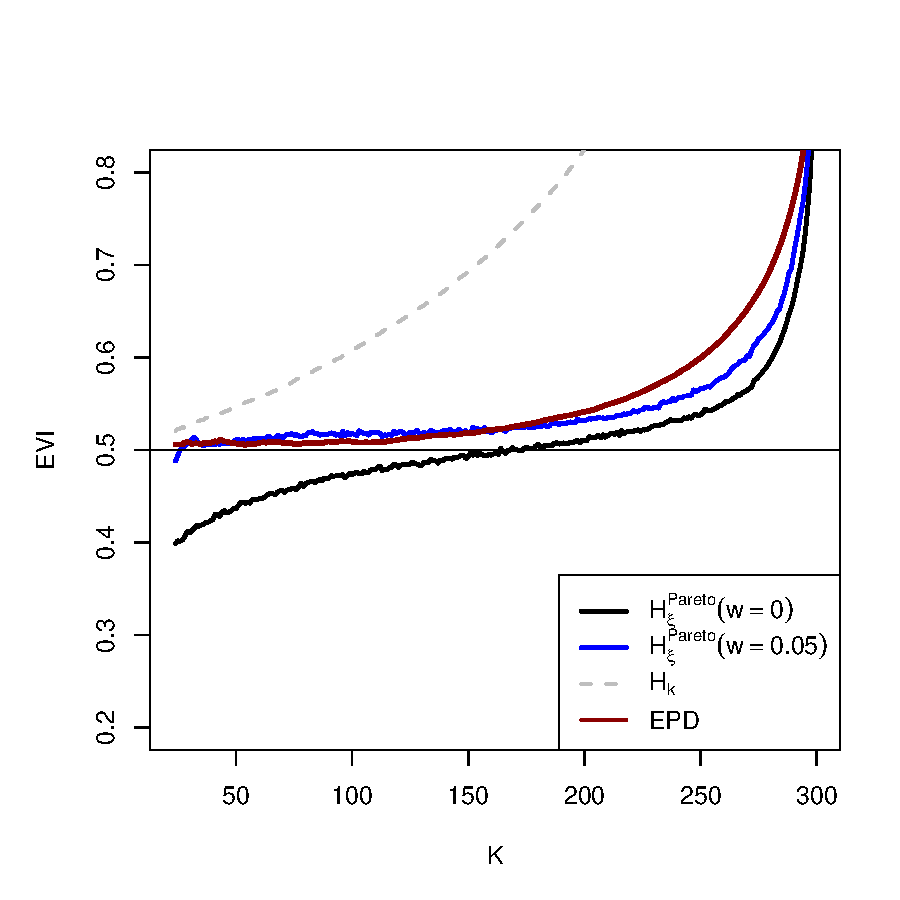
\includegraphics[width=0.47\textwidth]{EP_burr_xi_m24.pdf}
 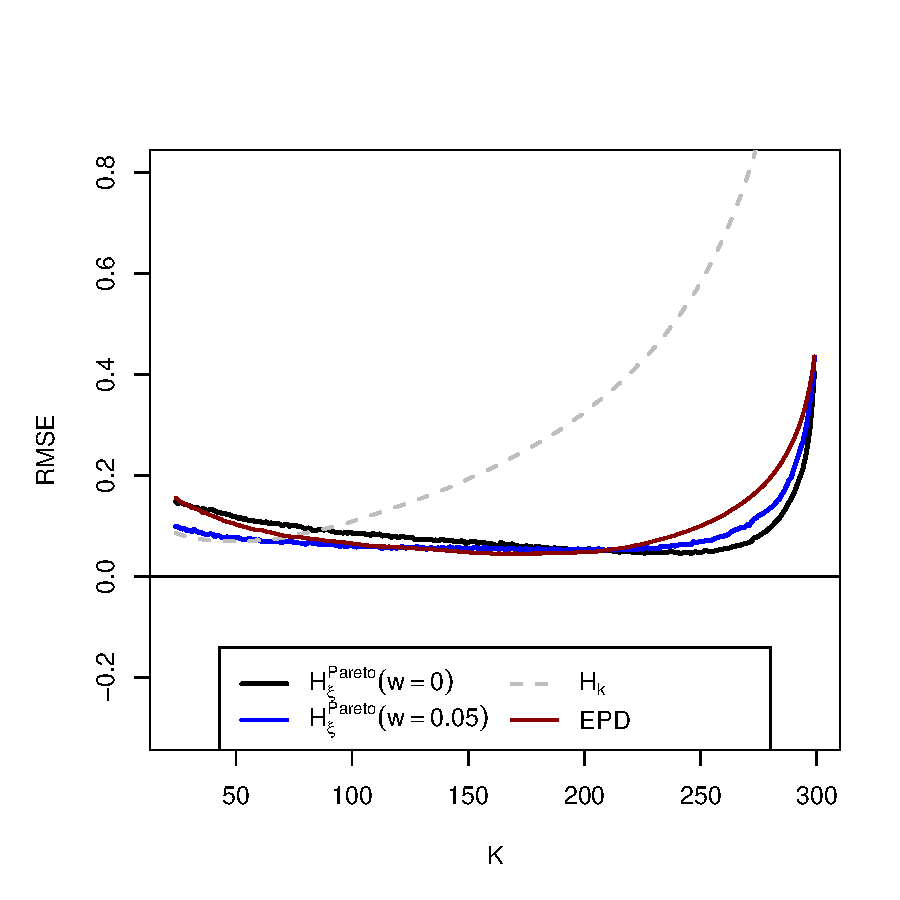
\includegraphics[width=0.47\textwidth]{EP_burr_rmse_m24.pdf}        
 \caption{\small Bias (left) and RMSE (right) of $\hat{\xi}$ for $X \sim$ Burr($\xi=0.5, \rho=-1$) using POT model $\hat{F}^{P}_t$} 
\end{figure}


\begin{figure}[!ht]
  \centering
 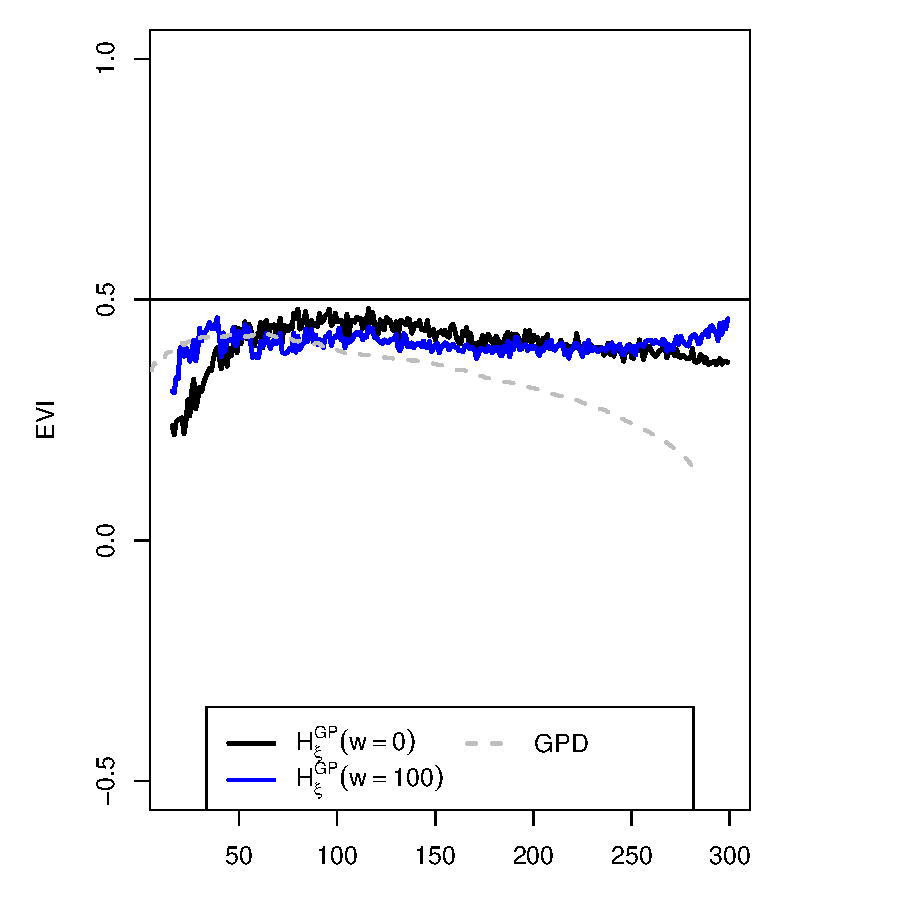
\includegraphics[width=0.47\textwidth]{EGP_burr_xi_m16.pdf}
 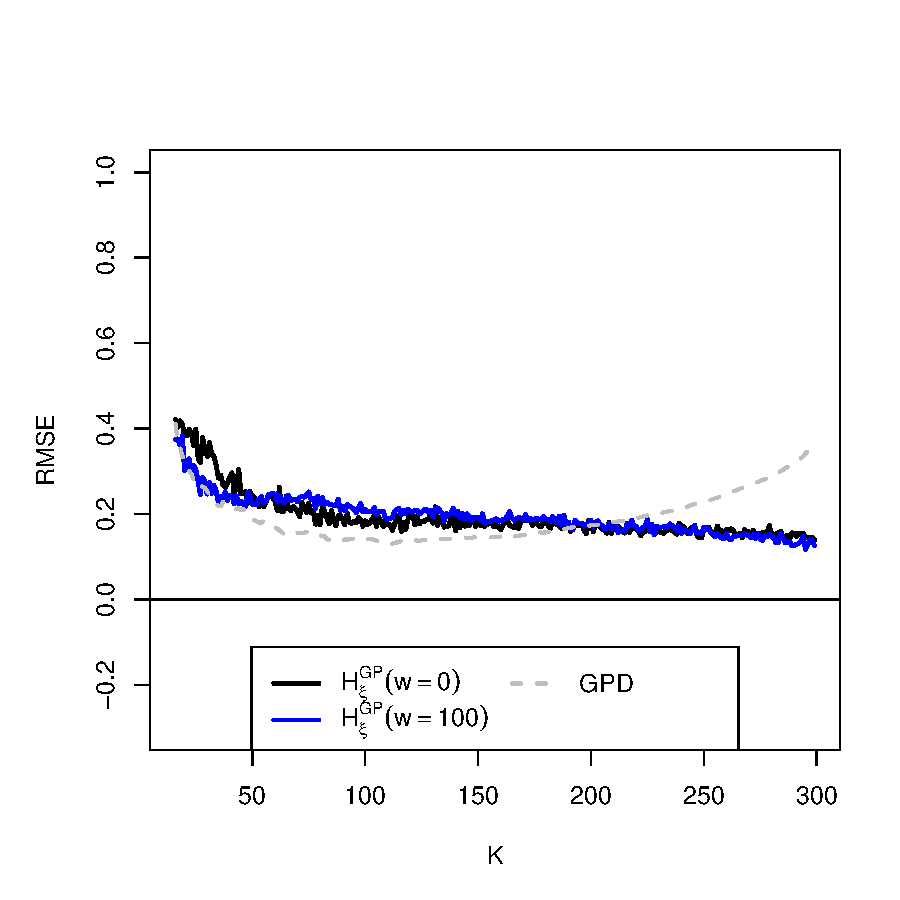
\includegraphics[width=0.47\textwidth]{EGP_burr_rmse_m16.pdf}        
\caption{\small Bias (left) and RMSE (right) of $\hat{\xi}$ for $X \sim$ Burr($\xi=0.5, \rho=-1$) using POT model $\hat{F}^{GP}_t$} 
 \end{figure}


\begin{figure}[!ht]
  \centering
 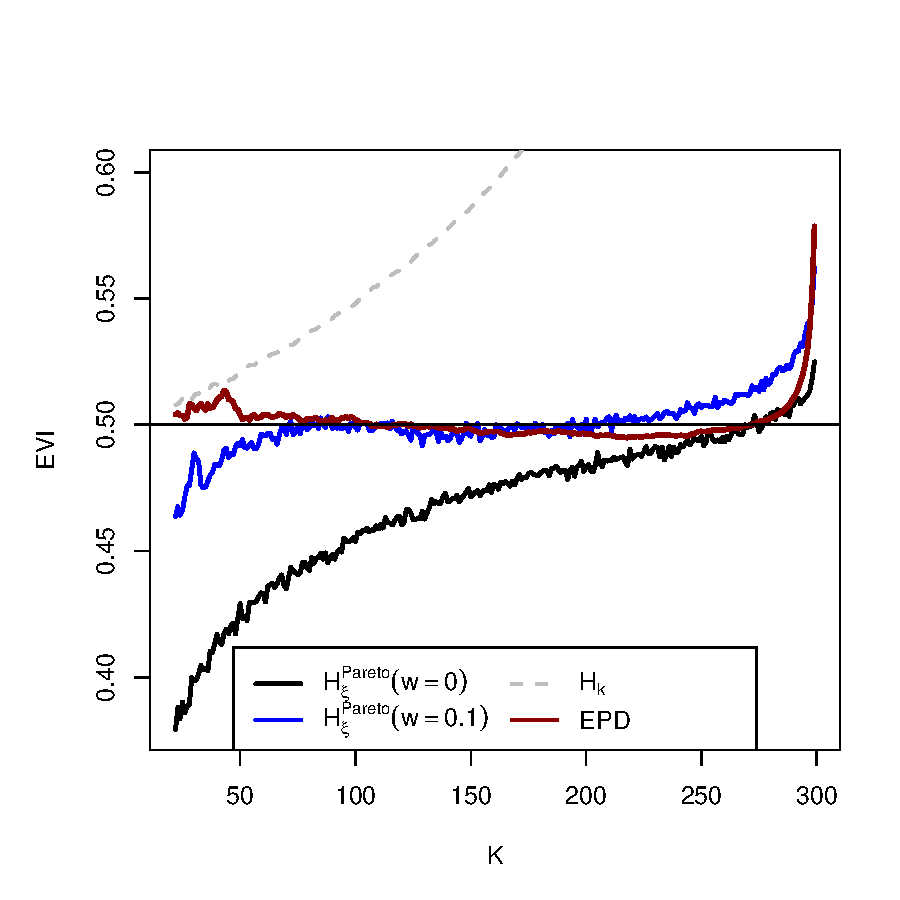
\includegraphics[width=0.47\textwidth]{EP_frechet_xi_m22.pdf}
 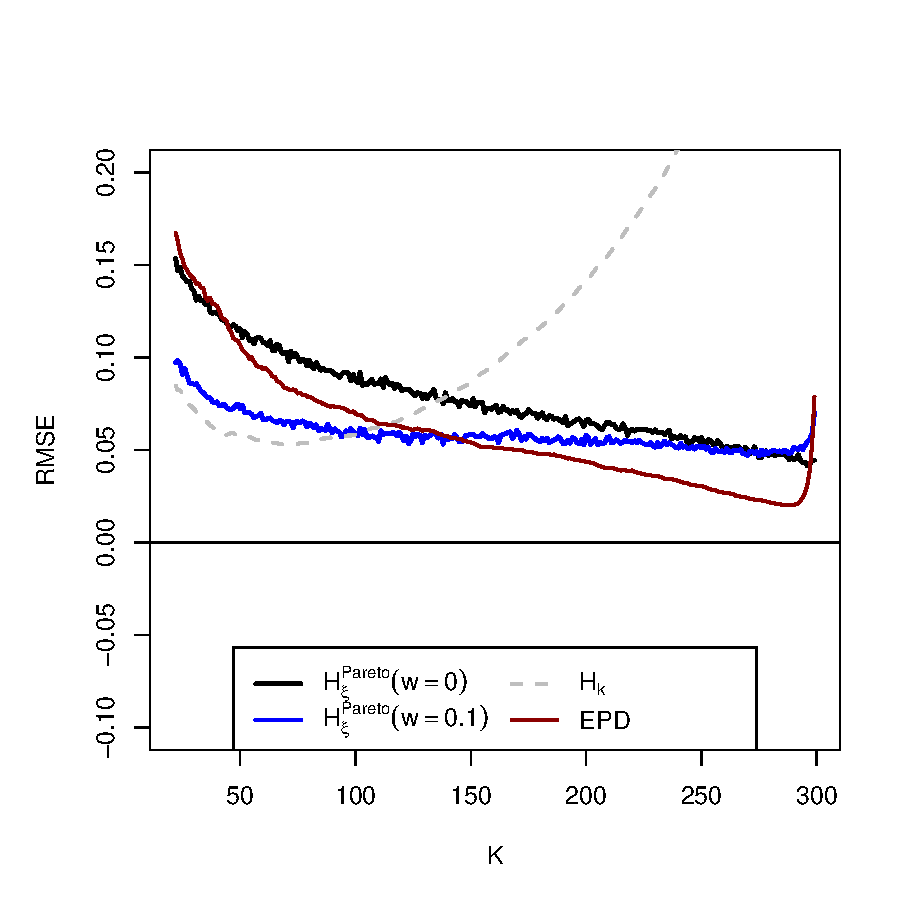
\includegraphics[width=0.47\textwidth]{EP_frechet_rmse_m22.pdf}       
\caption{\small Bias (left) and RMSE (right) of $\hat{\xi}$ for $X \sim$ Fr\'echet($\xi=0.5$) using POT model $\hat{F}^{P}_t$} 
 \end{figure}


\begin{figure}[!ht]
  \centering
 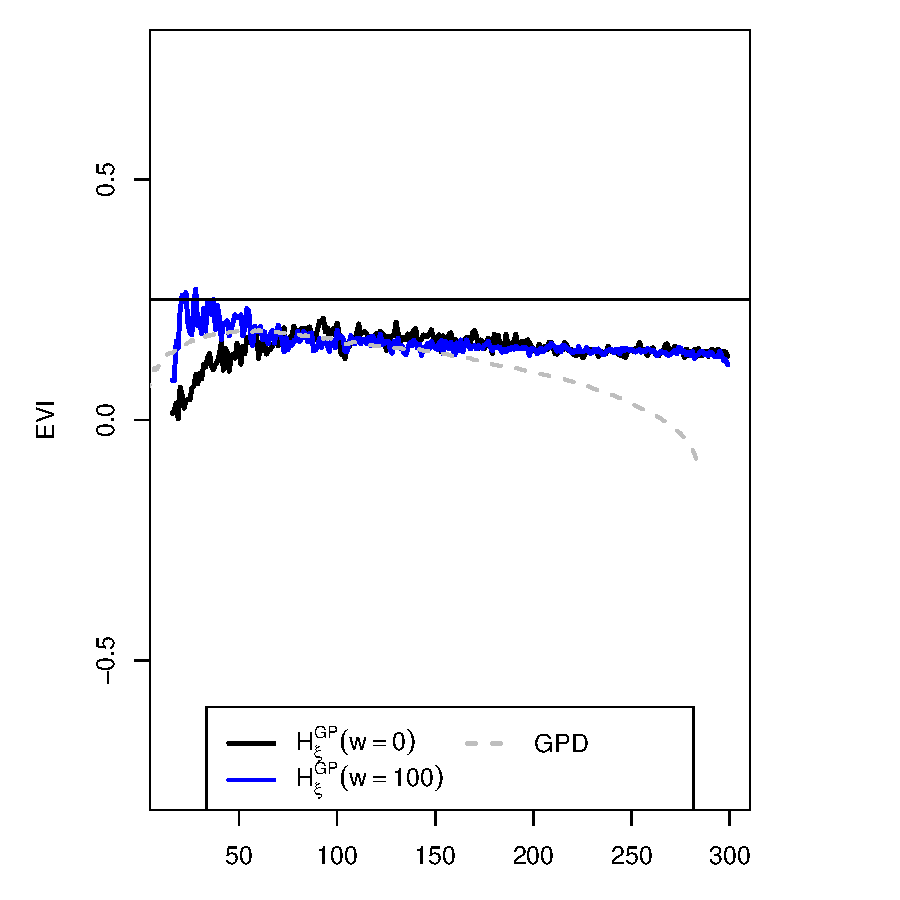
\includegraphics[width=0.47\textwidth]{EGP_frechet_xi_m16.pdf}
 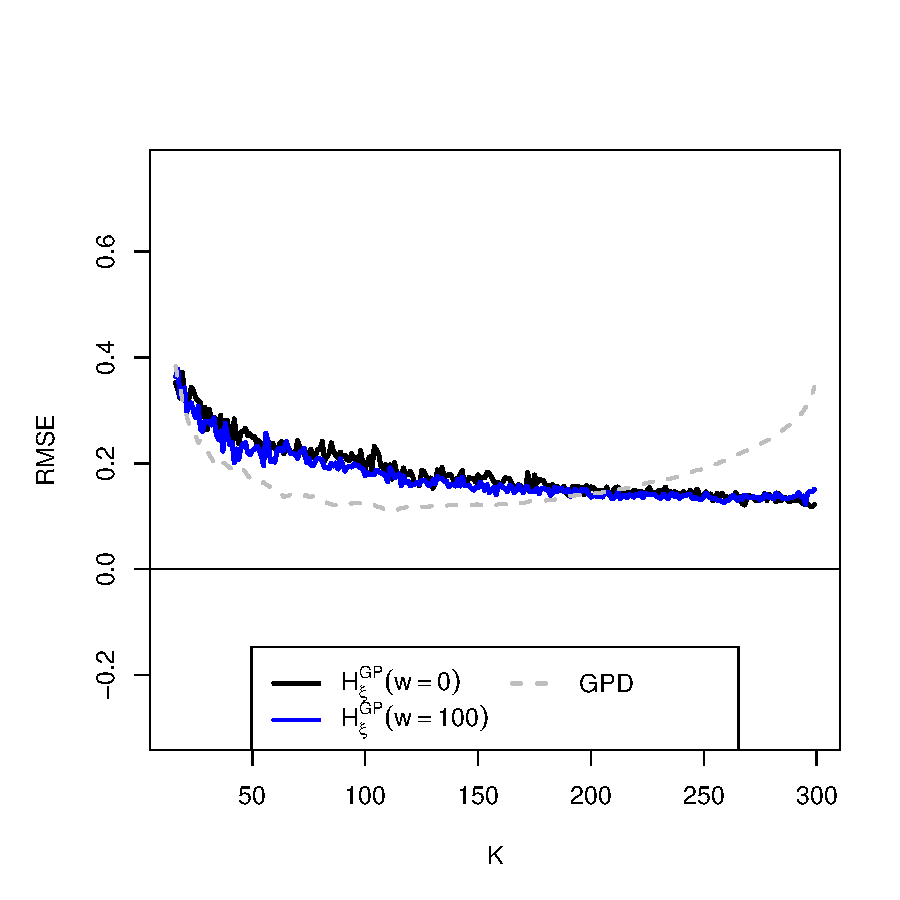
\includegraphics[width=0.47\textwidth]{EGP_frechet_rmse_m16.pdf}        
\caption{\small Bias (left) and RMSE (right) of $\hat{\xi}$ for $X \sim$ Fr\'echet($\xi=0.5$) using POT model $\hat{F}^{GP}_t$} 
 \end{figure}

\begin{figure}[!ht]
  \centering
 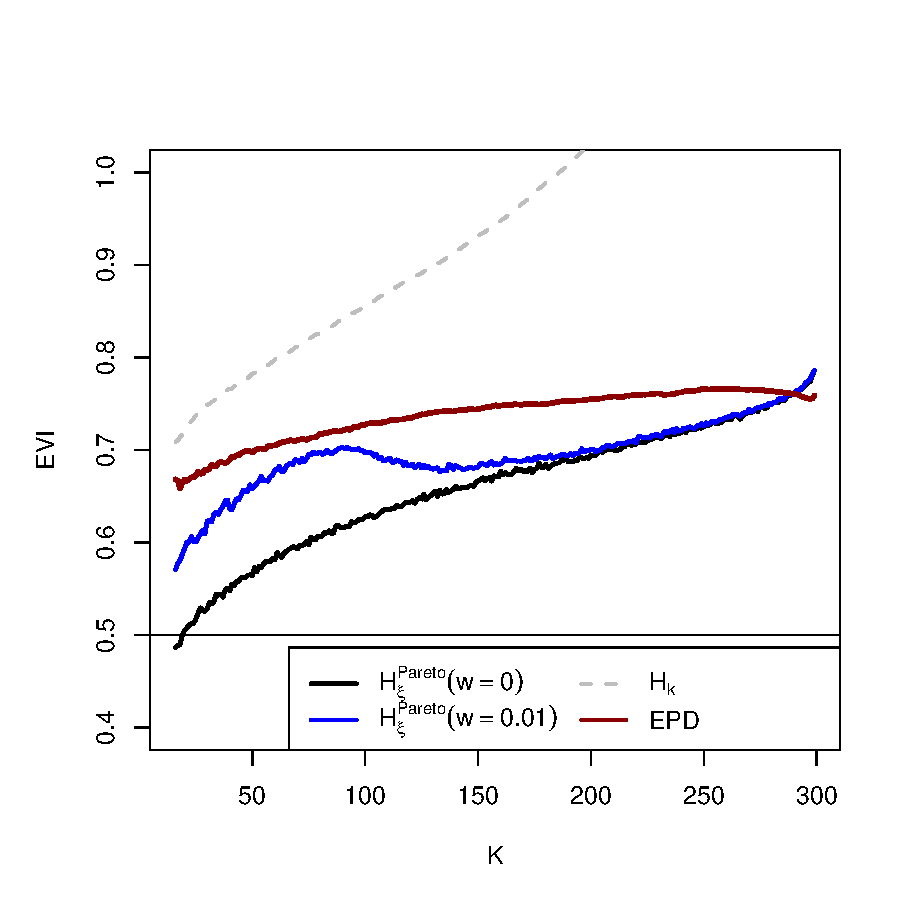
\includegraphics[width=0.47\textwidth]{EP_loggamma_xi_m16.pdf}
 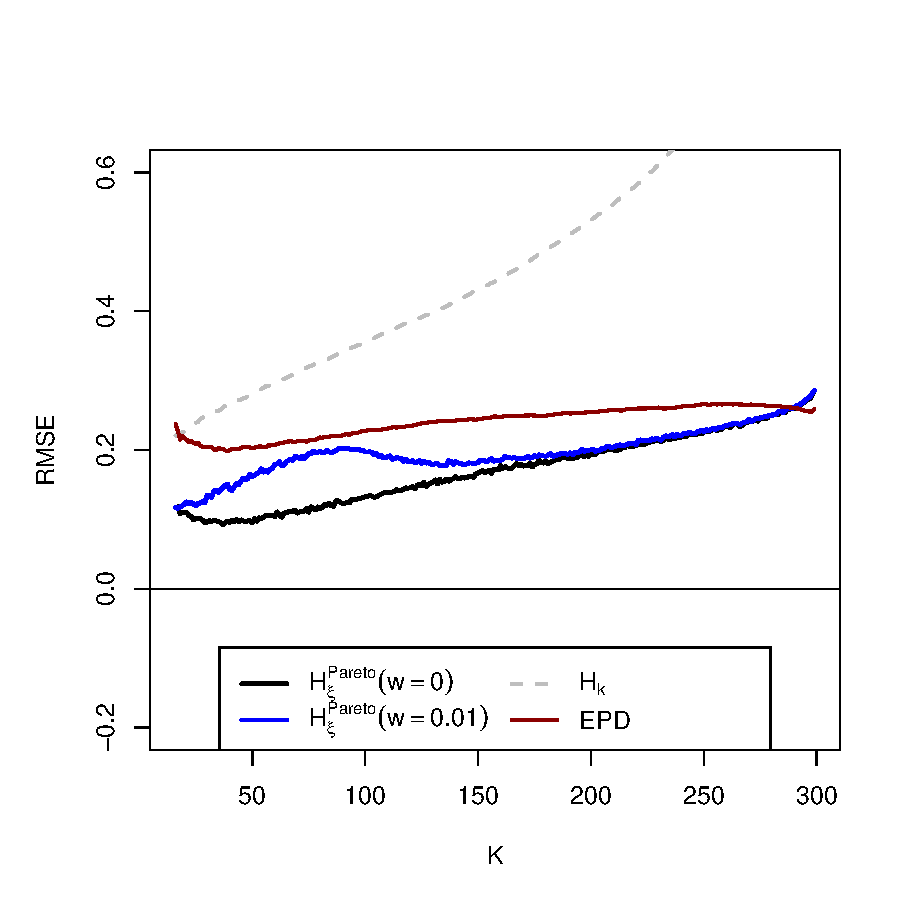
\includegraphics[width=0.47\textwidth]{EP_loggamma_rmse_m16.pdf}       
\caption{\small Bias (left) and RMSE (right) of $\hat{\xi}$ for $X \sim$ loggamma($\xi=0.5$) using POT model $\hat{F}^{P}_t$} 
 \end{figure}

\begin{figure}[!ht]
  \centering
  	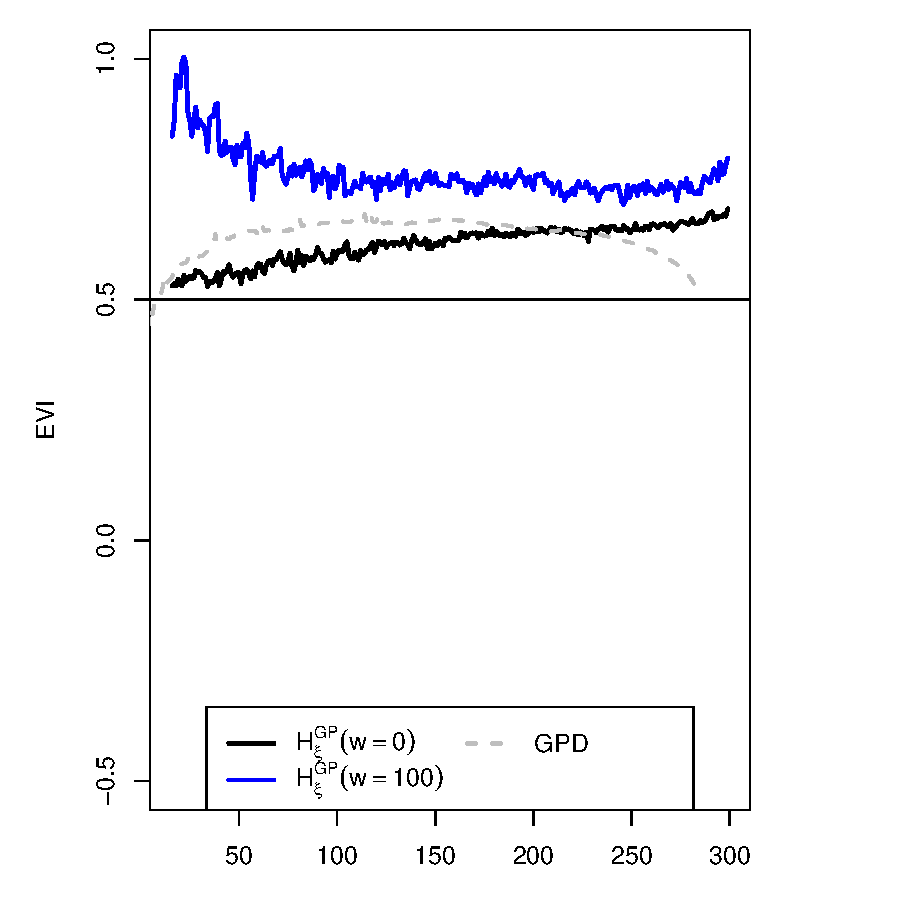
\includegraphics[width=0.47\textwidth]{EGP_loggamma_xi_m16.pdf}
  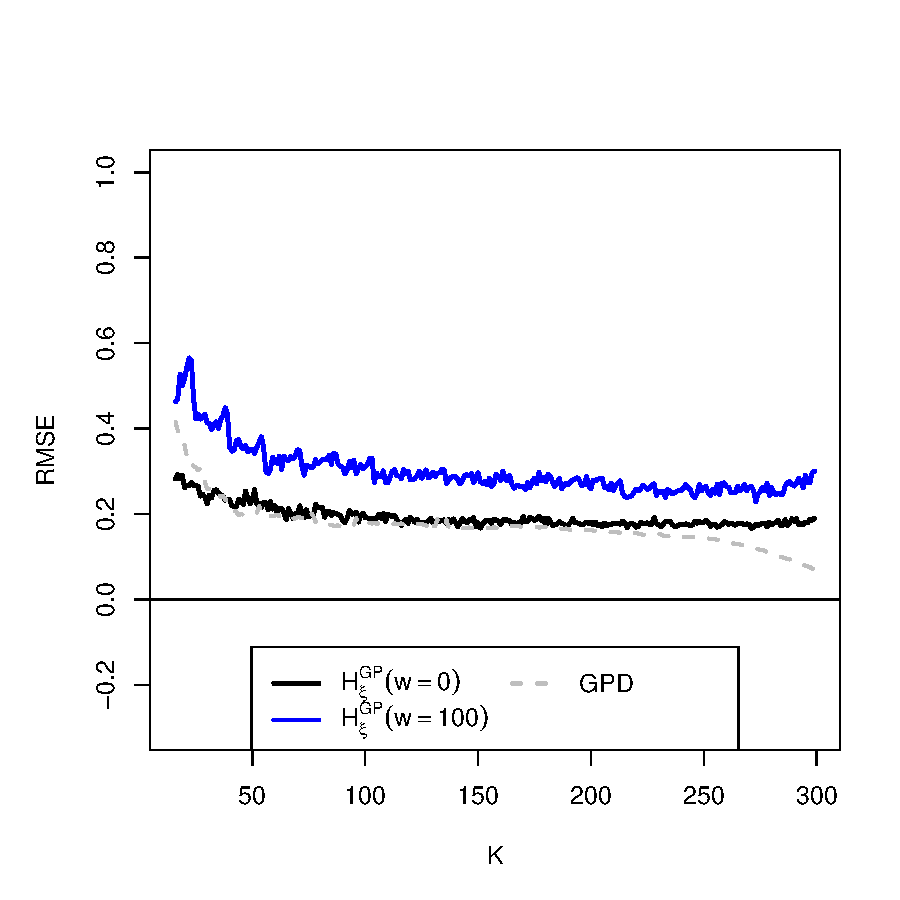
\includegraphics[width=0.47\textwidth]{EGP_loggamma_rmse_m16.pdf} 
\caption{\small Bias (left) and RMSE (right) of $\hat{\xi}$ for $X \sim$ loggamma($\xi=0.5$) using POT model $\hat{F}^{GP}_t$} 
 \end{figure}

\begin{figure}[!ht]
	\centering
 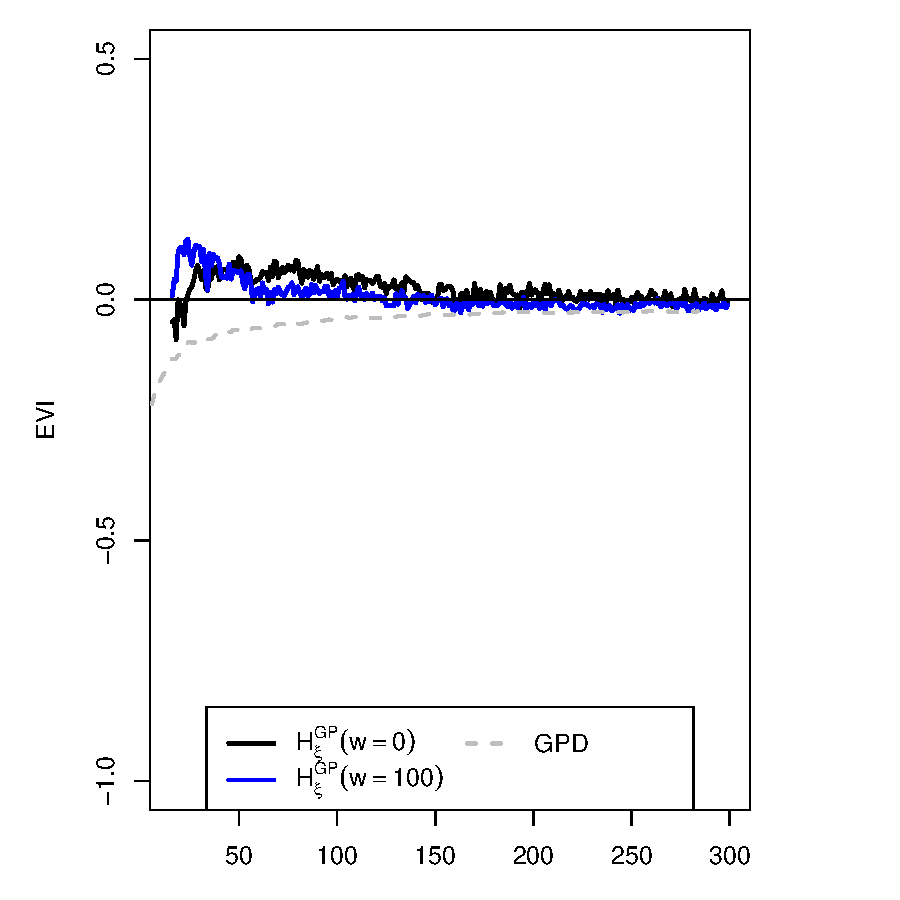
\includegraphics[width=0.47\textwidth]{EGP_gamma_xi_m16.pdf}
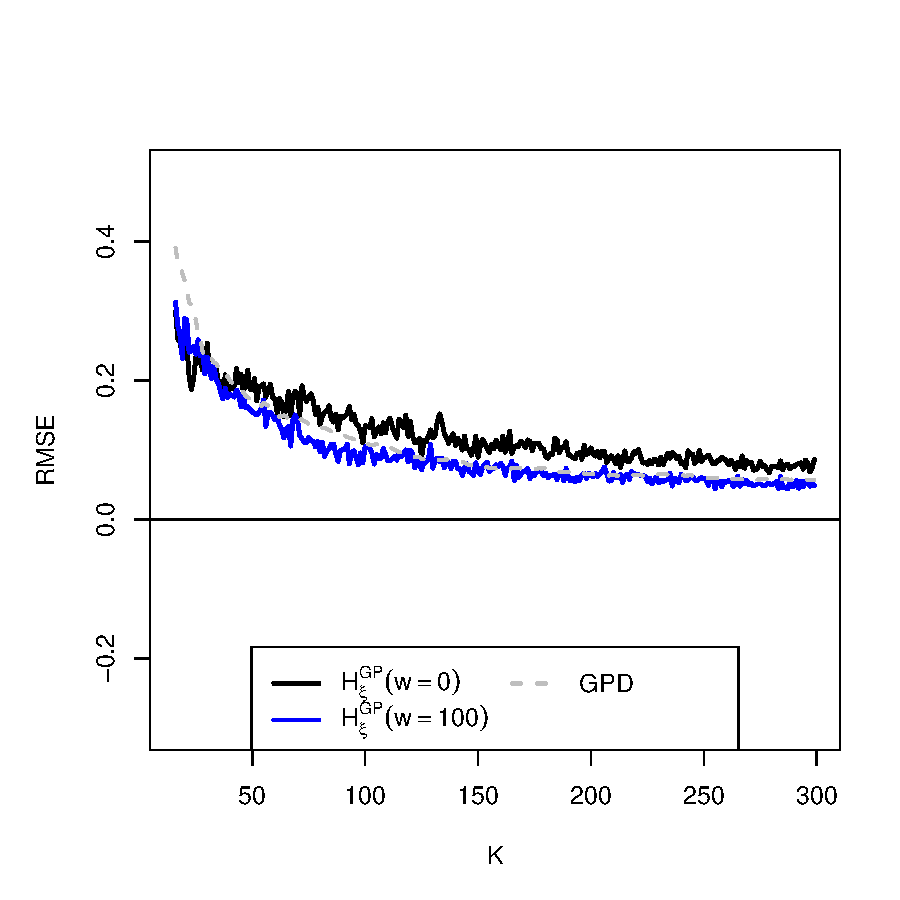
\includegraphics[width=0.47\textwidth]{EGP_gamma_rmse_m16.pdf}         
	\caption{\small Bias (left) and RMSE (right) of $\hat{\xi}$ for $X \sim$ Gamma($\xi=0$) using POT model $\hat{F}^{GP}_t$} 
\end{figure}

\begin{figure}[!ht]
	\centering
	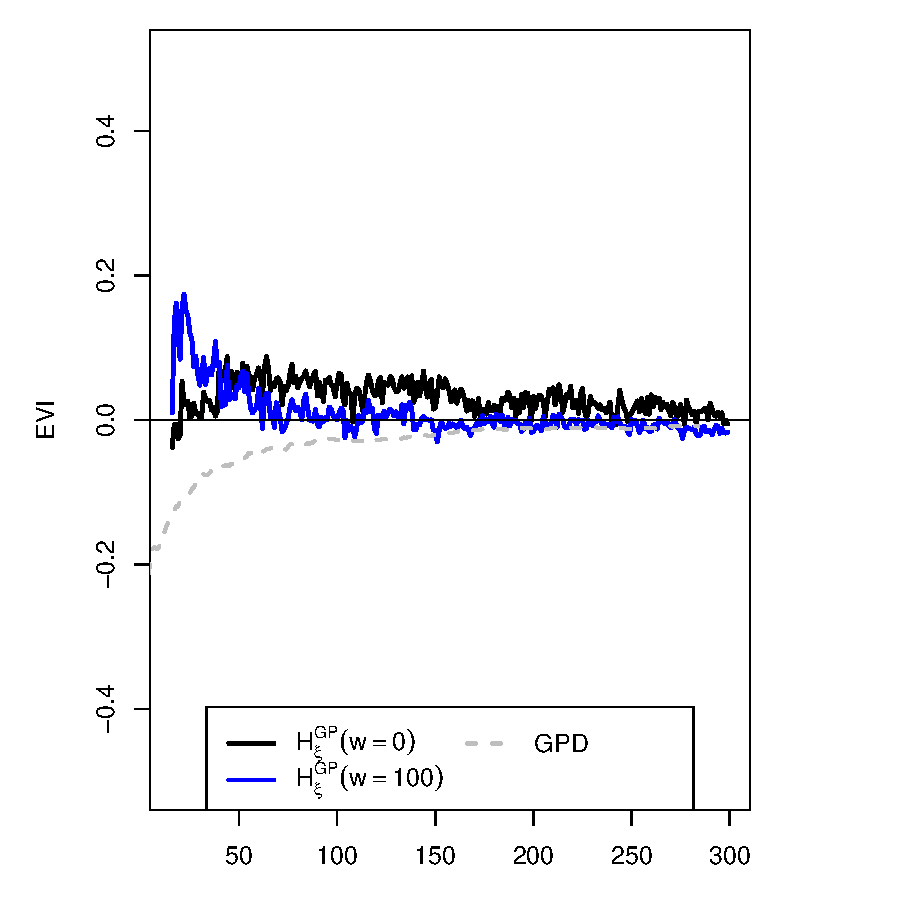
\includegraphics[width=0.47\textwidth]{EGP_exp_xi_m16.pdf}
	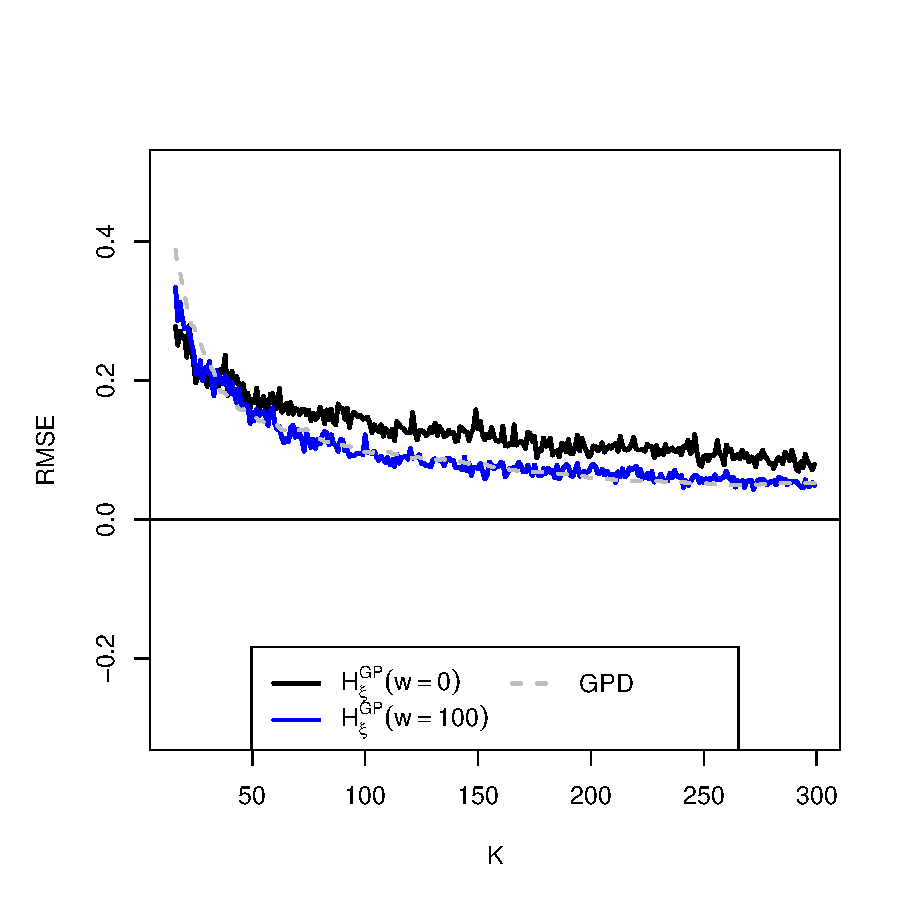
\includegraphics[width=0.47\textwidth]{EGP_exp_rmse_m16.pdf}        
	\caption{\small Bias (left) and RMSE (right) of $\hat{\xi}$ for $X \sim$ Exponential ($\xi=0$) using POT model $\hat{F}^{GP}_t$} 
\end{figure}

\begin{figure}[!ht]
	\centering
	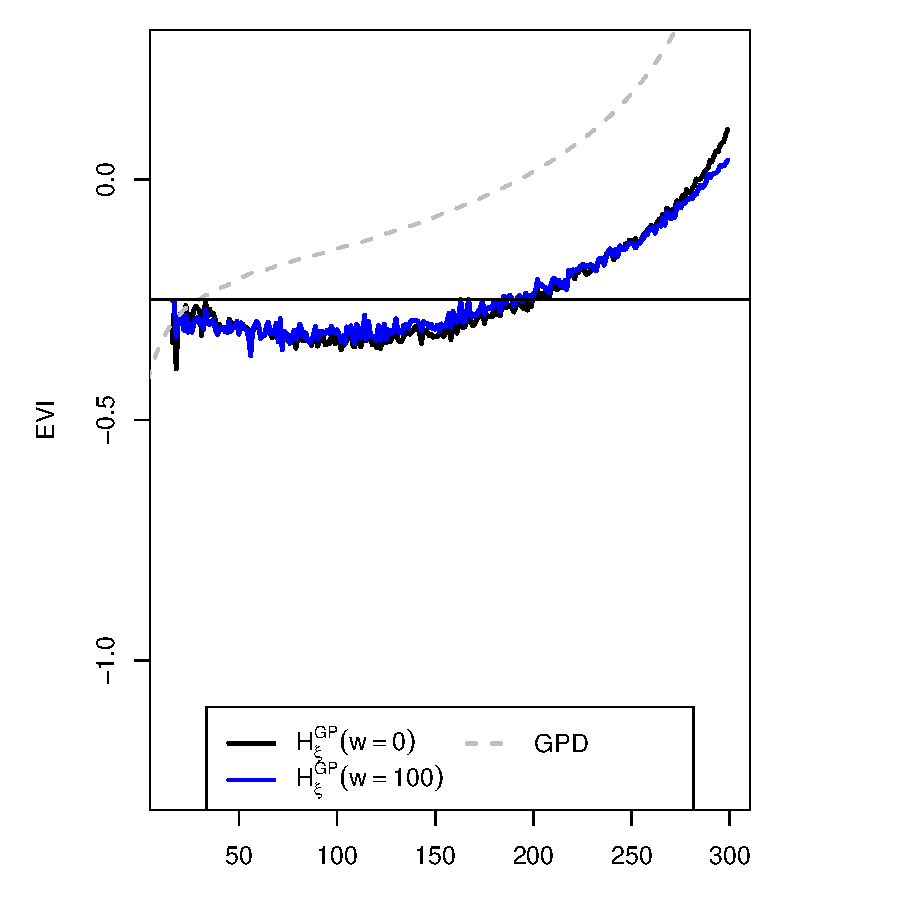
\includegraphics[width=0.47\textwidth]{EGP_beta_xi_m16.pdf}
	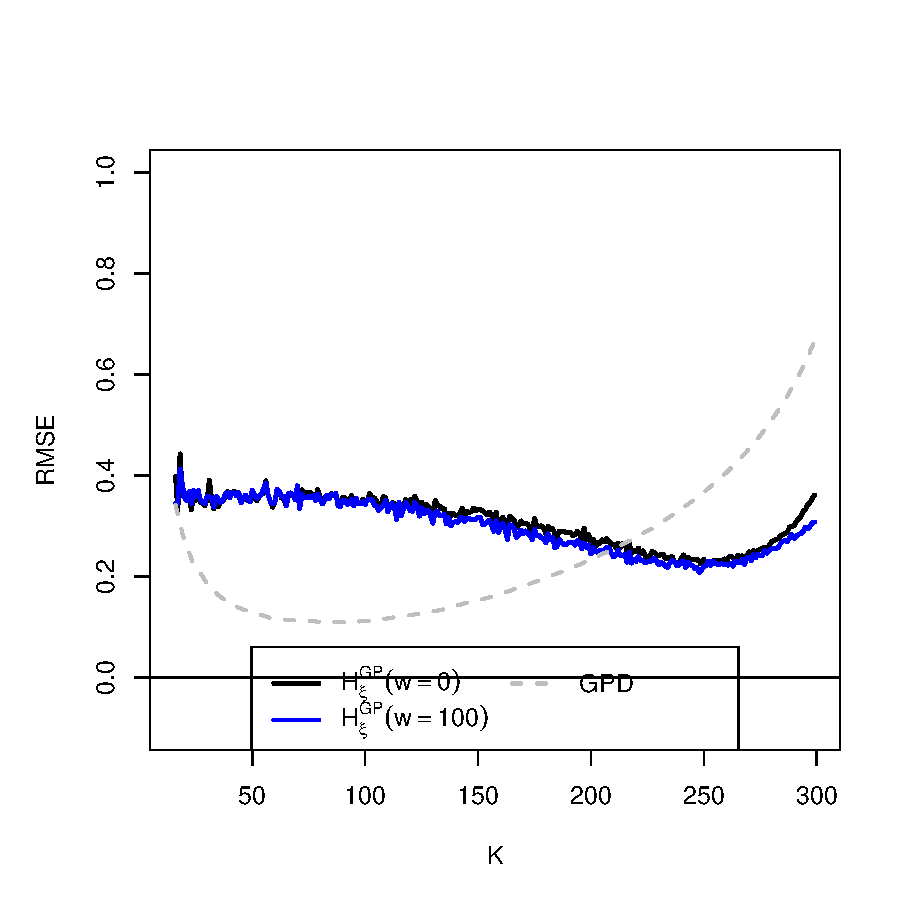
\includegraphics[width=0.47\textwidth]{EGP_beta_rmse_m16.pdf}        
	\caption{\small Bias (left) and RMSE (right) of $\hat{\xi}$ for $X \sim$ Beta ($\xi=-0.25$) using POT model $\hat{F}^{GP}_t$} 
\end{figure}


We end with a case study Motor Third Party Liability (MTPL) portfolio from a European country between 1995 and 2010. The data set contains 596 claims. 
All payments for a given claim relating to the same development year  aggregated in a single claim point, respectively incurred data point. We here use the ultimates, which contain the statistical forecasts in case of non-settled claims. From the mean excess plot it appears that several components exist in the ultimates distribution: while the mean excess first decreases, a linear increase is dominating, however first with a higher slope then ultimately for the largest ultimates. This suggests Pareto modelling with the extreme value index $\xi$ equal to the slope. The fitted models $\hat{F}^{GP}_t$ lead to estimates of $\xi$ which indeed show two distinct levels with a lower extreme value index for $k \leq 200$. Especially in case no penalization is applied in the estimation procedure the plot is extremely constant for $k > 200$ (except for the ultimate $k$ values or equivalently the lowest thresholds) which supports a three-component model approach. 
\begin{figure}[th]
	\centering
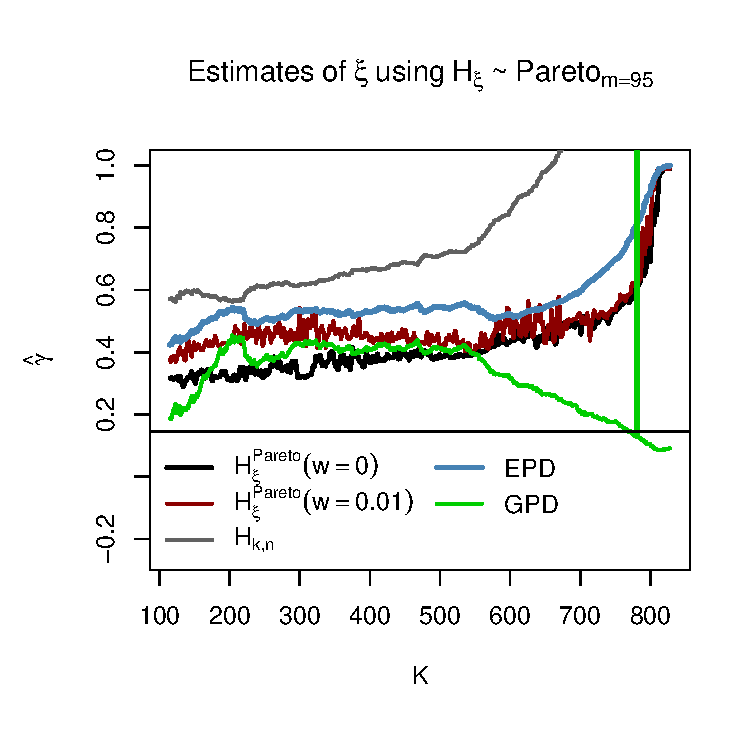
\includegraphics[width=0.47\textwidth]{xi_m95.pdf}        
	\caption{\small Penalized and non-penalized estimates of $\xi$ using POT model $\hat{F}^{P}_t$, jointly with Hill estimates $H_{k,n}$, GPD and EPD estimates based on POT model \eqref{EP}} 
\end{figure}

\begin{figure}[!ht]
  \centering
 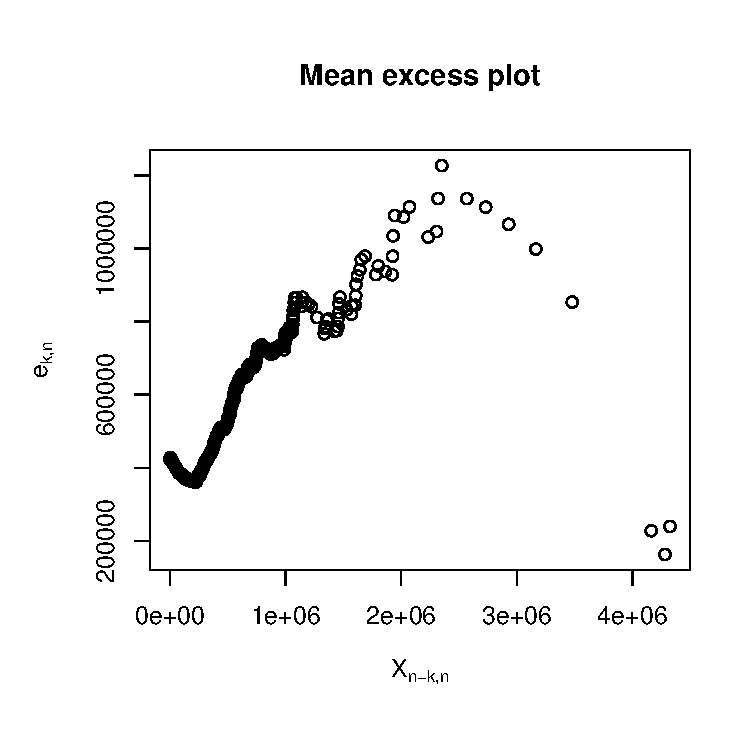
\includegraphics[width=0.47\textwidth]{CY2_MeanExcess.pdf}
 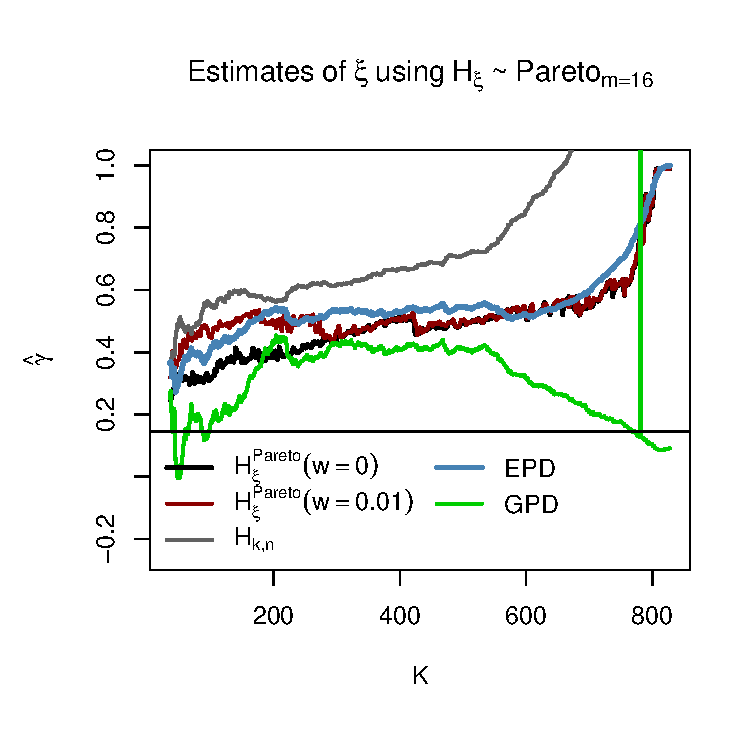
\includegraphics[width=0.47\textwidth]{xi_m16.pdf}        
\caption{\small Mean excess plot (left) and penalized ($w=0.01$) and non-penalized ($w=0$) estimates of $\xi$ using POT model $\hat{F}^{P}_t$, jointly with Hill estimates $H_{k,n}$ and EPD estimates based on POT model \eqref{EP}} 
 \end{figure}

\begin{figure}[hh!]
	\centering
	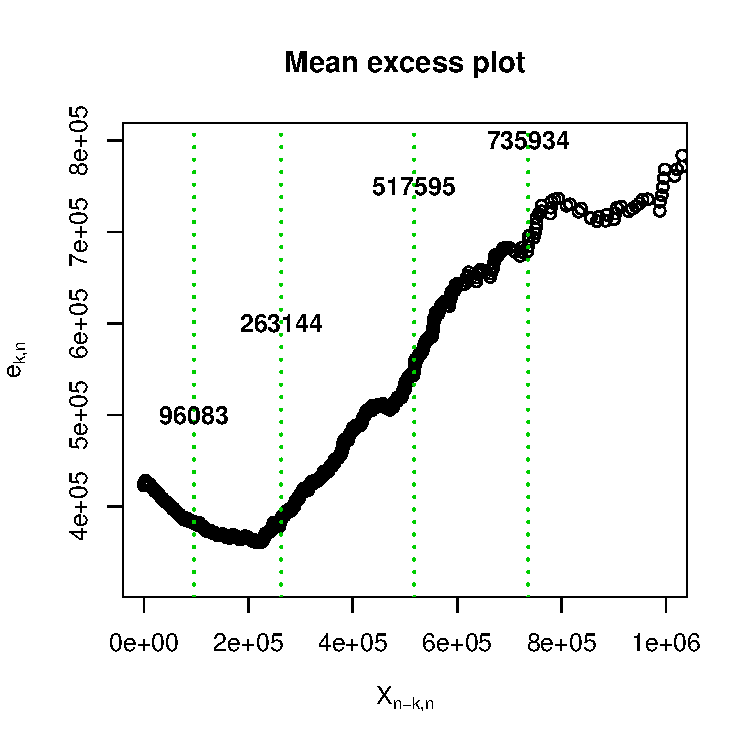
\includegraphics[width=0.47\textwidth]{thresh_MExcess_zoom_xi_m16.pdf}
	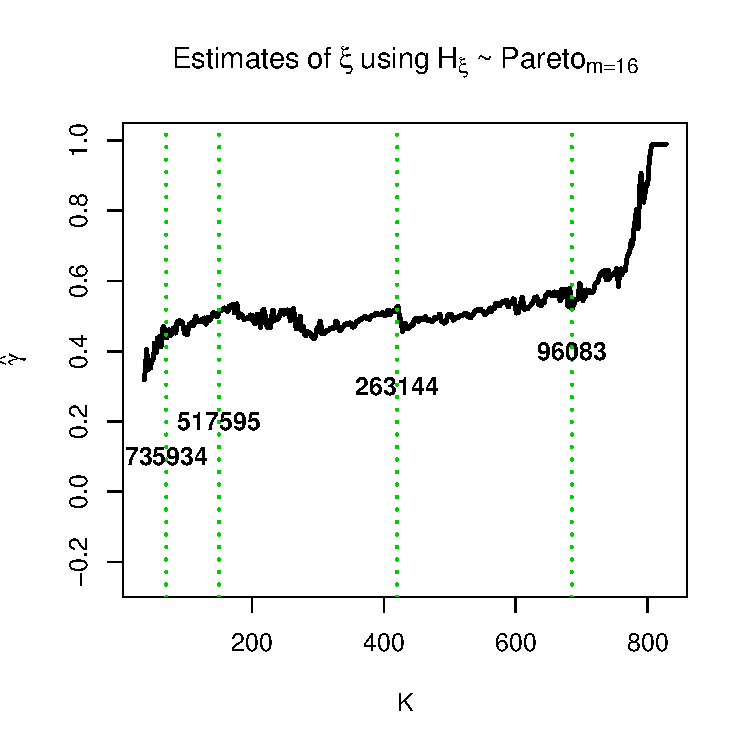
\includegraphics[width=0.47\textwidth]{thresh_xi_m16.pdf}        
	\caption{\small Zoomed Mean excess plot (left) and penalized ($w=0.01$) and non-penalized ($w=0$) estimates of $\xi$ using POT model $\hat{F}^{P}_t$, jointly with Hill estimates $H_{k,n}$, GPD and EPD estimates based on POT model \eqref{EP}} 
\end{figure}


\section{Acknowledgments}  
\label{Sec5}
	\noindent This work is based on the research supported wholly/in part by the National Research Foundation of South Africa (Grant Number 102628). The Grantholder acknowledges that opinions, findings and conclusions or recommendations expressed in any publication generated by the NRF supported research is that of the author(s), and that the NRF accepts no liability whatsoever in this regard. 

%\section{References}  
%\label{Sec6}
\begin{thebibliography}{99}
\bibitem{BDGM}
Beirlant, J., Dierckx, G., Goegebeur, Y. and  Matthys, G., 1999. Tail index estimation and an exponential regression model. {\it Extremes}, 2,157-180.

\bibitem{BDGS}
Beirlant, J., Dierckx, G, Guillou, A. and Starica, C., 2002. On exponential representations of log-spacings of extreme order statistics. {\it Extremes}, 5, 257-180.

\bibitem{BJS1}
Beirlant, J., Joossens, E. and Segers, J., 2002. Modelling excesses over high thresholds by perturbed generalized Pareto distributions. Eurandom Technical report.

\bibitem{BGTS}
Beirlant, J., Goegebeur, Y., Teugels, J. and Segers, J., 2004. {\it Statistics of Extremes: Theory and Applications}, Wiley, UK.

\bibitem{BJS2}
Beirlant, J., Joossens, E. and Segers, J., 2009.
 Second-order refined peaks-over-threshold modelling for heavy-tailed distributions. {\it Journal of Statistical Planning and Inference}, 139(8), 2800--2815.
 
 \bibitem{BMV}
Beirlant, J., Maribe, G. and Verster, A., 2017. Using shrinkage estimators to reduce bias and MSE in estimation of heavy tails. 
To appear in {\it Revstat}.

\bibitem{CG}
Caeiro, F. and Gomes, M.I., 2011. Semi-parametric tail inference through probability weighted moments. {\it J. Statist. Plann. Inference}, 141, 937-950.

\bibitem{D}
Drees, H., 1996. Refined pickands estimators wtth bias correction. {\it Communications in Statistics-Theory and Methods}, 25, 837-851.
 
 \bibitem{D}
 Dupuis, D., 1999. Exceedances over  high thresholds: A guide to threshold selection. {\it Extremes}, 1, 251--261.
 
 \bibitem{FH}
Feuerverger, A. and Hall, P., 1999. Estimating a tail exponent by modelling departure from a Pareto distribution. {\it Ann. Statist.}, 27, 760-781.  
 
\bibitem{FHR}
Frigessi, A., Haug, O.  and Rue, H., 2002.
  A dynamic mixture model for unsupervised tail estimation without threshold selection.{\it Extremes}, 5, 219--235.
  
  \bibitem{GMN}
  Gomes, M.I., Martins, M.J. and Neves, M., 2000. Alternatives to a semi-parametric estimator of parameters  of rare events - the Jackknife methodology. {\it Extremes}, 3, 207-229.
  
  \bibitem{GM}
  Gomes, M.I. and Martins, M.J., 2002. Asymptotically unbiased estimators of the tail index based on external estimation of the second order parameter. {\it Extremes}, 5, 5-31.
  
  \bibitem{HF}
de Haan, L. and Ferreira, A., 2006. {\it Extreme Value Theory: an Introduction}, Springer Science and Business Media, LLC, New York.  
  
\bibitem{H}
 Hill, B.M., 1975. A simple general approach about the tail of a distribution. {\it Annals of Statistics}, 3, 1163-1174.
 
 \bibitem{MB}
 Matthys, G. and Beirlant, J., 2000. Adaptive threshold selection in tail index estimation. Extremes and Integrated Risk Management, 37-49.

\bibitem{NHRH}
Naveau, P., Huser, R., Ribereau, P. and Hannart, A., 2016. Modeling jointly low, moderate and heavy rainfall intensities without a threshold selection. {\it Water Resour. Res. }, 52,
  2753--2769.

\bibitem{PT}
Papastathopoulos, I. and Tawn, J., 2013. Extended generalized Pareto models for tail estimation. {\it Journal of Statistical Planning and Inference}, 143, 131--143.

\bibitem{P}
Peng, L., 1998. Asymptotically unbiased estimator for the extreme-value index. {\it Statist. Prob. Lett.}, 38, 107-115.

\bibitem{PQ}
Peng, L. and Qi, Y., 2004. Estimating the first and second order parameters of a heavy tailed distribution. Australian \& New Zealand Journal of Statistics, 46(2), 305-312.
\end{thebibliography}		


\newpage
For the case where $H_{\xi} \sim Pareto$ we take a simple $Burr(\xi=0.5)$, first with $m=10$ and with $m=5$. Thus we expect the last weight $\omega_{m,m} = 1/m$ as $k \rightarrow 0$


\begin{table}[hh]
	\caption{Table of weights for $m=10$ where $\lambda = 0$}
	\centering
	\begin{tabular}{rrrrrrrrrrr}
		\hline
		& $\omega_1$ &  $\omega_2$ &  $\omega_3$ &  $\omega_4$ &  $\omega_5$ &  $\omega_6$ &  $\omega_7$ &  $\omega_8$ &  $\omega_9$ &  $\omega_10$ \\ 
		\hline
		K = 10 & 0.18 & 0.18 & 0.09 & 0.00 & 0.00 & 0.00 & 0.09 & 0.18 & 0.09 & 0.18 \\ 
		K = 11 & 0.25 & 0.17 & 0.08 & 0.00 & 0.00 & 0.00 & 0.08 & 0.17 & 0.08 & 0.17 \\ 
		K = 12 & 0.00 & 0.23 & 0.15 & 0.15 & 0.00 & 0.00 & 0.00 & 0.08 & 0.15 & 0.23 \\ 
		K = 13 & 0.00 & 0.07 & 0.21 & 0.14 & 0.14 & 0.00 & 0.00 & 0.00 & 0.07 & 0.36 \\ 
		K = 14 & 0.13 & 0.00 & 0.27 & 0.20 & 0.00 & 0.00 & 0.00 & 0.07 & 0.13 & 0.20 \\ 
		K = 15 & 0.00 & 0.19 & 0.00 & 0.25 & 0.12 & 0.06 & 0.00 & 0.00 & 0.06 & 0.31 \\ 
		K = 16 & 0.18 & 0.06 & 0.18 & 0.12 & 0.12 & 0.00 & 0.00 & 0.06 & 0.12 & 0.18 \\ 
		K = 17 & 0.00 & 0.00 & 0.11 & 0.17 & 0.28 & 0.11 & 0.00 & 0.06 & 0.11 & 0.17 \\ 
		K = 18 & 0.05 & 0.00 & 0.00 & 0.21 & 0.16 & 0.16 & 0.11 & 0.00 & 0.05 & 0.26 \\ 
		K = 19 & 0.10 & 0.00 & 0.00 & 0.10 & 0.15 & 0.25 & 0.10 & 0.00 & 0.05 & 0.25 \\ 
		&&&&&\dots\\
		K = 41 & 0.02 & 0.10 & 0.05 & 0.02 & 0.15 & 0.12 & 0.10 & 0.24 & 0.05 & 0.15 \\ 
		K = 42 & 0.00 & 0.00 & 0.05 & 0.10 & 0.02 & 0.05 & 0.14 & 0.17 & 0.17 & 0.31 \\ 
		K = 43 & 0.02 & 0.00 & 0.07 & 0.07 & 0.07 & 0.14 & 0.14 & 0.16 & 0.19 & 0.14 \\ 
		K = 44 & 0.05 & 0.00 & 0.05 & 0.09 & 0.07 & 0.14 & 0.16 & 0.16 & 0.16 & 0.14 \\ 
		K = 45 & 0.00 & 0.00 & 0.02 & 0.04 & 0.04 & 0.09 & 0.11 & 0.20 & 0.27 & 0.22 \\ 
		K = 46 & 0.00 & 0.00 & 0.00 & 0.02 & 0.02 & 0.04 & 0.13 & 0.11 & 0.28 & 0.39 \\ 
		K = 47 & 0.00 & 0.02 & 0.00 & 0.02 & 0.00 & 0.06 & 0.04 & 0.15 & 0.32 & 0.38 \\ 
		K = 48 & 0.00 & 0.02 & 0.02 & 0.00 & 0.02 & 0.00 & 0.10 & 0.15 & 0.31 & 0.38 \\ 
		K = 49 & 0.00 & 0.00 & 0.00 & 0.00 & 0.02 & 0.04 & 0.02 & 0.06 & 0.39 & 0.47 \\ 
		\hline
	\end{tabular}
\end{table}


\begin{table}[hh]
	\caption{Table of weights for $m=10$ where $\lambda = 1$}
	\centering
	\begin{tabular}{rrrrrrrrrrr}
		\hline
		& $\omega_1$ &  $\omega_2$ &  $\omega_3$ &  $\omega_4$ &  $\omega_5$ &  $\omega_6$ &  $\omega_7$ &  $\omega_8$ &  $\omega_9$ &  $\omega_10$ \\
		\hline
		K = 10 & 0.18 & 0.09 & 0.18 & 0.00 & 0.00 & 0.00 & 0.00 & 0.09 & 0.18 & 0.27 \\ 
		K = 11 & 0.25 & 0.08 & 0.17 & 0.00 & 0.00 & 0.00 & 0.00 & 0.08 & 0.17 & 0.25 \\ 
		K = 12 & 0.00 & 0.38 & 0.15 & 0.00 & 0.00 & 0.00 & 0.08 & 0.15 & 0.15 & 0.08 \\ 
		K = 13 & 0.07 & 0.29 & 0.21 & 0.00 & 0.00 & 0.00 & 0.07 & 0.14 & 0.14 & 0.07 \\ 
		K = 14 & 0.13 & 0.27 & 0.20 & 0.00 & 0.00 & 0.00 & 0.07 & 0.13 & 0.13 & 0.07 \\ 
		K = 15 & 0.12 & 0.06 & 0.31 & 0.12 & 0.00 & 0.00 & 0.06 & 0.12 & 0.06 & 0.12 \\ 
		K = 16 & 0.18 & 0.06 & 0.24 & 0.18 & 0.00 & 0.00 & 0.06 & 0.12 & 0.06 & 0.12 \\ 
		K = 17 & 0.00 & 0.00 & 0.11 & 0.17 & 0.28 & 0.11 & 0.00 & 0.06 & 0.11 & 0.17 \\ 
		K = 18 & 0.05 & 0.00 & 0.11 & 0.16 & 0.26 & 0.11 & 0.00 & 0.05 & 0.11 & 0.16 \\ 
		K = 19 & 0.10 & 0.00 & 0.20 & 0.20 & 0.20 & 0.00 & 0.00 & 0.10 & 0.10 & 0.10 \\ 
		&&&&&\dots\\
		K = 41 & 0.05 & 0.07 & 0.07 & 0.10 & 0.15 & 0.12 & 0.12 & 0.17 & 0.05 & 0.10 \\ 
		K = 42 & 0.00 & 0.05 & 0.10 & 0.07 & 0.12 & 0.14 & 0.14 & 0.24 & 0.02 & 0.12 \\ 
		K = 43 & 0.02 & 0.05 & 0.09 & 0.05 & 0.07 & 0.19 & 0.12 & 0.23 & 0.07 & 0.12 \\ 
		K = 44 & 0.05 & 0.00 & 0.09 & 0.07 & 0.05 & 0.23 & 0.11 & 0.20 & 0.09 & 0.11 \\ 
		K = 45 & 0.00 & 0.00 & 0.04 & 0.02 & 0.09 & 0.09 & 0.16 & 0.20 & 0.27 & 0.13 \\ 
		K = 46 & 0.00 & 0.00 & 0.02 & 0.00 & 0.07 & 0.09 & 0.11 & 0.24 & 0.35 & 0.13 \\ 
		K = 47 & 0.00 & 0.02 & 0.00 & 0.02 & 0.06 & 0.06 & 0.13 & 0.30 & 0.28 & 0.13 \\ 
		K = 48 & 0.00 & 0.02 & 0.02 & 0.02 & 0.00 & 0.06 & 0.17 & 0.25 & 0.33 & 0.12 \\ 
		K = 49 & 0.00 & 0.00 & 0.00 & 0.02 & 0.04 & 0.02 & 0.06 & 0.29 & 0.45 & 0.12 \\ 
		\hline
	\end{tabular}
\end{table}



\begin{table}[hh]
	\caption{Table of weights for $m=5$ where $\lambda = 0$}
	\centering
	\begin{tabular}{rrrrrr}
		\hline
		& $\omega_1$ &  $\omega_2$ &  $\omega_3$ &  $\omega_4$ &  $\omega_5$ \\
		\hline
		K = 5 & 0.00 & 0.00 & 0.17 & 0.33 & 0.50 \\ 
		K = 6 & 0.14 & 0.00 & 0.14 & 0.29 & 0.43 \\ 
		K = 7 & 0.25 & 0.00 & 0.12 & 0.25 & 0.38 \\ 
		K = 8 & 0.33 & 0.00 & 0.00 & 0.33 & 0.33 \\ 
		K = 9 & 0.40 & 0.00 & 0.10 & 0.20 & 0.30 \\ 
		K = 10 & 0.27 & 0.18 & 0.00 & 0.09 & 0.45 \\ 
		K = 11 & 0.33 & 0.17 & 0.00 & 0.08 & 0.42 \\ 
		K = 12 & 0.38 & 0.15 & 0.00 & 0.23 & 0.23 \\ 
		K = 13 & 0.14 & 0.43 & 0.00 & 0.07 & 0.36 \\ 
		K = 14 & 0.33 & 0.27 & 0.00 & 0.07 & 0.33 \\ 
		&&&&&\dots\\
		K = 36 & 0.06 & 0.19 & 0.25 & 0.33 & 0.17 \\ 
		K = 37 & 0.11 & 0.16 & 0.24 & 0.32 & 0.16 \\ 
		K = 38 & 0.11 & 0.18 & 0.24 & 0.32 & 0.16 \\ 
		K = 39 & 0.13 & 0.18 & 0.23 & 0.31 & 0.15 \\ 
		K = 40 & 0.10 & 0.07 & 0.28 & 0.35 & 0.20 \\ 
		K = 41 & 0.12 & 0.12 & 0.27 & 0.34 & 0.15 \\ 
		K = 42 & 0.00 & 0.14 & 0.12 & 0.31 & 0.43 \\ 
		K = 43 & 0.02 & 0.14 & 0.12 & 0.30 & 0.42 \\ 
		K = 44 & 0.05 & 0.14 & 0.11 & 0.30 & 0.41 \\ 
		K = 45 & 0.00 & 0.07 & 0.16 & 0.29 & 0.49 \\ 
		K = 46 & 0.00 & 0.02 & 0.11 & 0.39 & 0.48 \\ 
		K = 47 & 0.02 & 0.02 & 0.06 & 0.32 & 0.57 \\ 
		K = 48 & 0.02 & 0.02 & 0.02 & 0.25 & 0.69 \\ 
		K = 49 & 0.00 & 0.00 & 0.06 & 0.12 & 0.82 \\ 
		\hline
	\end{tabular}
\end{table}


\begin{table}[hh]
	\caption{Table of weights for $m=5$ where $\lambda = 1$}
	\centering
	\begin{tabular}{rrrrrr}
		\hline
		& $\omega_1$ &  $\omega_2$ &  $\omega_3$ &  $\omega_4$ &  $\omega_5$ \\
		\hline
		K = 5 & 0.00 & 0.00 & 0.17 & 0.33 & 0.50 \\ 
		K = 6 & 0.14 & 0.00 & 0.14 & 0.29 & 0.43 \\ 
		K = 7 & 0.25 & 0.00 & 0.12 & 0.38 & 0.25 \\ 
		K = 8 & 0.33 & 0.00 & 0.11 & 0.33 & 0.22 \\ 
		K = 9 & 0.40 & 0.00 & 0.10 & 0.20 & 0.30 \\ 
		K = 10& 0.45 & 0.00 & 0.09 & 0.18 & 0.27 \\ 
		K = 11& 0.50 & 0.00 & 0.00 & 0.25 & 0.25 \\ 
		K = 12 & 0.38 & 0.15 & 0.00 & 0.23 & 0.23 \\ 
		K = 13 & 0.29 & 0.29 & 0.00 & 0.21 & 0.21 \\ 
		K = 14 & 0.33 & 0.27 & 0.00 & 0.20 & 0.20 \\ 
		&&&&&\dots\\
		K = 36 & 0.06 & 0.17 & 0.28 & 0.31 & 0.19 \\ 
		K = 37 & 0.08 & 0.16 & 0.27 & 0.30 & 0.19 \\ 
		K = 38 & 0.11 & 0.18 & 0.24 & 0.32 & 0.16 \\ 
		K = 39 & 0.13 & 0.15 & 0.21 & 0.31 & 0.21 \\ 
		K = 40 & 0.10 & 0.12 & 0.22 & 0.35 & 0.20 \\ 
		K = 41 & 0.12 & 0.10 & 0.27 & 0.34 & 0.17 \\ 
		K = 42 & 0.05 & 0.14 & 0.26 & 0.36 & 0.19 \\ 
		K = 43 & 0.07 & 0.14 & 0.26 & 0.35 & 0.19 \\ 
		K = 44 & 0.05 & 0.18 & 0.25 & 0.34 & 0.18 \\ 
		K = 45 & 0.02 & 0.09 & 0.27 & 0.40 & 0.22 \\ 
		K = 46 & 0.02 & 0.07 & 0.20 & 0.52 & 0.20 \\ 
		K = 47 & 0.02 & 0.04 & 0.21 & 0.45 & 0.28 \\ 
		K = 48 & 0.02 & 0.04 & 0.10 & 0.46 & 0.38 \\ 
		K = 49 & 0.00 & 0.02 & 0.06 & 0.24 & 0.67 \\ 
		\hline
	\end{tabular}
\end{table}



\end{document}